\section{对偶问题与最优性证书}
\label{sec:opt-con-duality}

KKT条件检验的是一个候选点，回答“它是否满足最优点应有的关系”。实际求解时还需要另一种回答：给定一个可行点，它的目标值离最优值最多差多少。可行点只给出最优值的上界，要控制差距，必须另有下界。上一节的乘子正好能产生下界：把约束乘以合法乘子加进目标，就得到一个在可行域上不超过原目标的函数。本节固定原问题，研究这种下界怎样构造、什么时候能一直提高到原最优值，以及怎样把原始和对偶两侧的候选合成一份证书；问题数据改变时最优值怎样变化，放到下一节讨论。

\subsection{对偶函数与弱对偶}
\label{sec:opt-con-weak-duality}

\paragraph{先对原变量取下确界}
固定$\bm\lambda\geq\bm0$和任意$\bm\nu$。对每个可行点$\bm x$，$\lambda_ig_i(\bm x)\leq0$、$h_j(\bm x)=0$，所以$\mathcal L(\bm x,\bm\lambda,\bm\nu)\leq f(\bm x)$。如果再对全体$\bm x\in\mathbb R^d$（不论是否可行）取下确界，得到的数不会超过任何可行点的目标值。

\begin{definition}[对偶函数与对偶问题]
\label{def:opt-con-dual-function}
问题~\eqref{eq:opt-con-problem}的\term{对偶函数}（dual function）为
\[
  q(\bm\lambda,\bm\nu)=\inf_{\bm x\in\mathbb R^d}\mathcal L(\bm x,\bm\lambda,\bm\nu),
\]
允许取$-\infty$。称$\max\{q(\bm\lambda,\bm\nu):\bm\lambda\geq\bm0\}$为\term{对偶问题}（dual problem），其最优值记为$d^\star=\sup_{\bm\lambda\geq\bm0,\bm\nu}q(\bm\lambda,\bm\nu)$。满足$\bm\lambda\geq\bm0$且$q(\bm\lambda,\bm\nu)>-\infty$的乘子称为对偶可行。
\end{definition}

对每个固定的$\bm x$，$\mathcal L(\bm x,\cdot,\cdot)$是乘子的仿射函数；$q$是这族仿射函数的逐点下确界，因而无论原问题是否凸，$q$总是凹函数，对偶问题总是凸问题。

\begin{theorem}[弱对偶]
\label{thm:opt-con-weak-duality}
对任意可行$\bm x$与任意$\bm\lambda\geq\bm0$、$\bm\nu$，有$q(\bm\lambda,\bm\nu)\leq f(\bm x)$。因而$d^\star\leq f^\star$。
\end{theorem}

\begin{proof}
$q(\bm\lambda,\bm\nu)\leq\mathcal L(\bm x,\bm\lambda,\bm\nu)\leq f(\bm x)$，第一步是下确界的定义，第二步是上面的符号论证。对可行$\bm x$取下确界、对乘子取上确界即得$d^\star\leq f^\star$。
\end{proof}

\term{弱对偶}（weak duality）不需要凸性、可微性或约束资格。两值都有限时，差$f^\star-d^\star\geq0$称为\term{对偶间隙}（duality gap）。

\paragraph{一个可以画出来的下界}
考虑$\min x^2$、约束$g(x)=1-x\leq0$，最优点$x^\star=1$，$f^\star=1$。$\mathcal L(x,\lambda)=x^2+\lambda(1-x)$在$x=\lambda/2$处取最小，于是$q(\lambda)=\lambda-\lambda^2/4$，在$\lambda=2$处达到$d^\star=1=f^\star$。图~\ref{fig:opt-con-dual-envelope}给出这个计算的几何含义。把每个$x$映成平面点$(u,t)=(g(x),f(x))$，得到曲线$G$；对固定的$\lambda$，$\mathcal L=t+\lambda u$在直线$t+\lambda u=\text{常数}$上不变，这族直线的斜率都是$-\lambda$。$q(\lambda)$就是把斜率为$-\lambda$的直线从下方推到刚好碰到$G$时，直线在$u=0$处的截距。原问题要求$u=g(x)\leq0$，最优值是$G$中$u\leq0$部分的最低高度；每条支撑直线在$u=0$处的截距都不超过它，这就是弱对偶。对偶问题在所有斜率中寻找截距最高的一条，本例中$\lambda=2$的直线恰好在$(0,1)$处与$G$相切。

\begin{figure*}[!htbp]
  \centering
  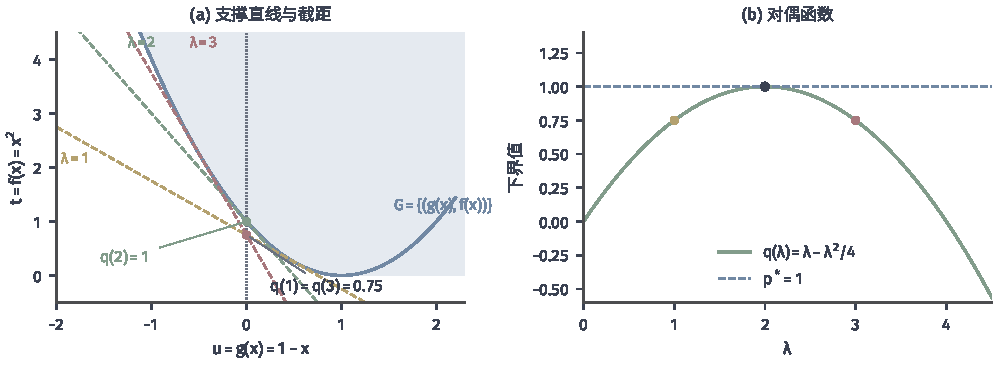
\includegraphics[width=169mm]{figures/03-optimization-evolution-and-signals/01-optimization/matplotlib/c5-dual-envelope/figure.pdf}
  \caption{$\min x^2$、$1-x\leq0$的对偶函数。(a) 蓝色曲线为$G=\{(1-x,x^2)\}$，浅蓝区域为其右上方的点；三条虚线是斜率为$-\lambda$（$\lambda=1,2,3$）且从下方接触$G$的直线，它们在$u=0$的截距即$q(\lambda)$。$\lambda=1$与$\lambda=3$的截距同为$0.75$，$\lambda=2$的截距为$1$，与原最优值相等。(b) 对偶函数$q(\lambda)=\lambda-\lambda^2/4$是凹函数，始终位于$f^\star=1$下方，最大值在$\lambda=2$处达到。}
  \label{fig:opt-con-dual-envelope}
\end{figure*}

在等式二次例中同样可以显式计算：$\mathcal L=\frac12(x_1^2+4x_2^2)+\nu(x_1+x_2-1)$在$x_1=-\nu$、$x_2=-\nu/4$处取最小，$q(\nu)=-\frac58\nu^2-\nu$，在$\nu^\star=-4/5$处达到$d^\star=2/5=f^\star$。对偶函数也可能处处为$-\infty$：在$[-1,1]$上最小化$-x^2$时，$\mathcal L=-x^2+\lambda_1(x-1)+\lambda_2(-x-1)$对任何乘子都没有下界，所以$d^\star=-\infty$，而$f^\star=-1$。某一组乘子给出$q=-\infty$，只说明这组乘子没有提供有用的下界。

\paragraph{近似内层只给出上方估计}
计算$q(\bm\lambda,\bm\nu)$本身是一个无约束最小化。若内层只算到近似点$\tilde{\bm x}$，那么$\mathcal L(\tilde{\bm x},\bm\lambda,\bm\nu)\geq q(\bm\lambda,\bm\nu)$，这个数在真正的下界上方，不能直接当作原问题的下界。要得到可靠下界，必须扣除一个经过证明的内层误差$\varepsilon$。例如$\mathcal L(\cdot,\bm\lambda,\bm\nu)$为$\mu$强凸时，对任意$\bm y$，
\[
  \mathcal L(\bm y)\geq\mathcal L(\tilde{\bm x})+\langle\nabla\mathcal L(\tilde{\bm x}),\bm y-\tilde{\bm x}\rangle+\frac\mu2\lVert\bm y-\tilde{\bm x}\rVert_2^2\geq\mathcal L(\tilde{\bm x})-\frac{1}{2\mu}\lVert\nabla\mathcal L(\tilde{\bm x})\rVert_2^2,
\]
最后一步对$\bm y$最小化右端的二次函数。于是$\mathcal L(\tilde{\bm x})-\lVert\nabla_{\bm x}\mathcal L(\tilde{\bm x})\rVert_2^2/(2\mu)$是可信下界。没有这类误差界时，近似内层值只能作为启发性估计。

\paragraph{原始—对偶间隙证书}
把两侧合起来，就得到可以交给别人核对的证书。若$\hat{\bm x}$可行、$(\bm\lambda,\bm\nu)$满足$\bm\lambda\geq\bm0$，则由弱对偶，
\begin{equation}
\label{eq:opt-con-gap-certificate}
  q(\bm\lambda,\bm\nu)\leq f^\star\leq f(\hat{\bm x}),\qquad
  0\leq f(\hat{\bm x})-f^\star\leq f(\hat{\bm x})-q(\bm\lambda,\bm\nu).
\end{equation}
右端可以计算，不需要知道$f^\star$。在等式二次例中取可行点$\hat{\bm x}=(3/4,1/4)^\top$与乘子$\nu=-3/4$：$f(\hat{\bm x})=0.40625$，$q(-3/4)=-\frac58\cdot\frac9{16}+\frac34=0.3984375$，间隙为$0.0078125$，所以$\hat{\bm x}$的次优性不超过$0.0079$；实际次优性为$0.40625-0.4=0.00625$。报告这样的证书时应分别给出三项：$\hat{\bm x}$的原始可行性（约束残差）、乘子的合法性（$\bm\lambda\geq\bm0$且$q$的计算可信），以及上下界之差。任何一项缺失，式~\eqref{eq:opt-con-gap-certificate}都不能使用。

第~\ref{chap:opt-linear-programming}章的线性规划对偶是这一构造的特例。对标准型$\min\bm c^\top\bm x$、$\bm A\bm x=\bm b$、$\bm x\geq\bm0$，把$-\bm x\leq\bm0$的乘子记为$\bm s\geq\bm0$、等式乘子记为$-\bm y$，则$\mathcal L=\bm c^\top\bm x-\bm y^\top(\bm A\bm x-\bm b)-\bm s^\top\bm x=\bm b^\top\bm y+(\bm c-\bm A^\top\bm y-\bm s)^\top\bm x$。关于$\bm x$的下确界有限当且仅当$\bm c-\bm A^\top\bm y-\bm s=\bm0$，此时$q=\bm b^\top\bm y$；消去$\bm s\geq\bm0$即得对偶问题$\max\bm b^\top\bm y$、$\bm A^\top\bm y\leq\bm c$。线性规划的特殊之处在于内层可以显式消去，本节保留的是同一个“用价格给目标作下界”的问题。

\subsection{凸共轭与对偶表示}
\label{sec:opt-con-conjugate}

对偶函数的计算核心是“目标加一个线性项后取下确界”。这一运算单独拿出来就是凸共轭。它把目标函数、约束集合与下方仿射函数联系起来，也为下一小节证明强对偶准备了工具。

\paragraph{用仿射函数从下方逼近}
设$f:\mathbb R^d\to\mathbb R\cup\{+\infty\}$。固定斜率$\bm y$，问：截距至少要降多少，仿射函数$\langle\bm y,\bm x\rangle-\beta$才能处处不超过$f$？条件是$\beta\geq\langle\bm y,\bm x\rangle-f(\bm x)$对所有$\bm x$成立，最小的$\beta$就是下面的上确界。

\begin{definition}[凸共轭]
\label{def:opt-con-conjugate}
函数$f$的\term{凸共轭}（convex conjugate）为$f^*(\bm y)=\sup_{\bm x\in\mathbb R^d}\{\langle\bm y,\bm x\rangle-f(\bm x)\}$，取值于$\mathbb R\cup\{+\infty\}$；$f(\bm x)=+\infty$的点不影响上确界。
\end{definition}

于是$\langle\bm y,\bm x\rangle-f^*(\bm y)$是斜率为$\bm y$的最高仿射下界，它的截距是$-f^*(\bm y)$。$f^*$是一族仿射函数（以$\bm x$为参数）的上确界，所以总是凸的，即使$f$不凸。由定义直接得到\term{Fenchel--Young不等式}（Fenchel--Young inequality）
\begin{equation}
\label{eq:opt-con-fenchel-young}
  f(\bm x)+f^*(\bm y)\geq\langle\bm x,\bm y\rangle\qquad\text{对所有}\ \bm x,\bm y.
\end{equation}

\begin{example}[几个基本共轭]
\label{ex:opt-con-conjugates}
(1) $f(x)=x^2/2$：$yx-x^2/2=y^2/2-(x-y)^2/2$在$x=y$处最大，故$f^*(y)=y^2/2$；斜率$y$的最高下界$yx-y^2/2$在$x=y$处与抛物线相切。更一般地，$\bm Q\succ\bm0$时$f(\bm x)=\frac12\bm x^\top\bm Q\bm x$的共轭为$\frac12\bm y^\top\bm Q^{-1}\bm y$，最大点满足$\bm Q\bm x=\bm y$。

(2) 范数$f(\bm x)=\lVert\bm x\rVert$：记对偶范数$\lVert\bm y\rVert_*=\sup_{\lVert\bm x\rVert\leq1}\langle\bm y,\bm x\rangle$。若$\lVert\bm y\rVert_*\leq1$，则$\langle\bm y,\bm x\rangle\leq\lVert\bm x\rVert$，上确界在$\bm x=\bm0$处取到$0$；若$\lVert\bm y\rVert_*>1$，存在$\bm x$使$\langle\bm y,\bm x\rangle>\lVert\bm x\rVert$，沿$t\bm x$放大得$+\infty$。故$f^*=\iota_{\{\lVert\bm y\rVert_*\leq1\}}$。例如$\lVert\cdot\rVert_1$的共轭是$\ell_\infty$单位球的指示函数。

(3) 设$C$是闭凸集，其\term{指示函数}（indicator function）$\iota_C$的共轭为$\iota_C^*(\bm y)=\sup_{\bm x\in C}\langle\bm y,\bm x\rangle$，称为$C$的\term{支撑函数}（support function），记为$\sigma_C(\bm y)$。它给出集合$C$沿方向$\bm y$伸出多远。
\end{example}

图~\ref{fig:opt-con-conjugate}画出前两个例子。左图中斜率$y=1.5$的直线$yx$向下平移$f^*(1.5)=1.125$后与抛物线相切，红色线段的长度就是最大竖直间隔$yx-x^2/2$。右图中绝对值函数只容许斜率$|y|\leq1$的直线从原点处支撑；斜率$1.5$的直线在$x>0$一侧无论怎样下移，最终都会越过$|x|$，所以$f^*(1.5)=+\infty$。例~\ref{ex:opt-con-conjugates}的(2)(3)两条合起来说明：范数的共轭是单位球的指示函数，指示函数的共轭是支撑函数，惩罚项与硬约束在共轭下互相转换。

\begin{figure*}[!htbp]
  \centering
  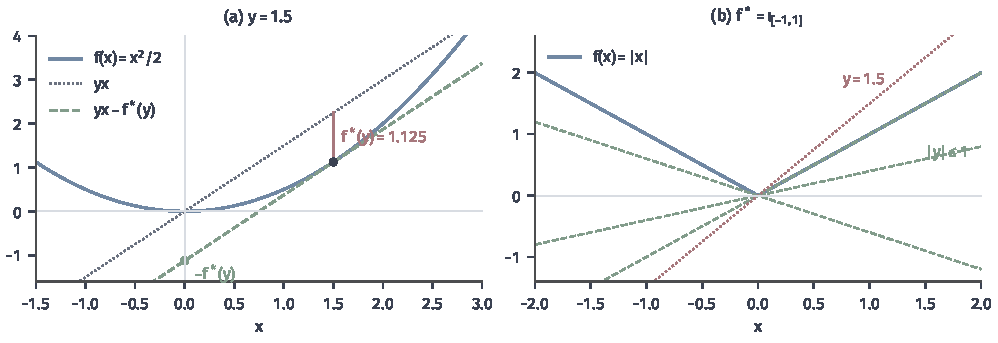
\includegraphics[width=169mm]{figures/03-optimization-evolution-and-signals/01-optimization/matplotlib/c5-conjugate/figure.pdf}
  \caption{共轭是最高仿射下界的截距。(a) $f(x)=x^2/2$，灰色点线为$yx$（$y=1.5$），绿色虚线为把它下移$f^*(y)=1.125$后的切线，红色线段是两者在$x=y$处的竖直间隔，绿点为截距$-f^*(y)$。(b) $f(x)=|x|$，绿色虚线为斜率$-0.6,0.4,1$的支撑直线，都经过原点；红色点线斜率为$1.5$，在$x>0$处超过$f$，不能平移成下界，故$f^*=\iota_{[-1,1]}$。}
  \label{fig:opt-con-conjugate}
\end{figure*}

共轭可以直接写出对偶函数。对线性等式约束问题$\min f(\bm x)$、$\bm A\bm x=\bm b$，
\[
  \begin{aligned}
    q(\bm\nu)&=\inf_{\bm x}\{f(\bm x)+\bm\nu^\top(\bm A\bm x-\bm b)\}
    =-\sup_{\bm x}\{\langle-\bm A^\top\bm\nu,\bm x\rangle-f(\bm x)\}-\bm b^\top\bm\nu\\
    &=-f^*(-\bm A^\top\bm\nu)-\bm b^\top\bm\nu.
  \end{aligned}
\]
等式二次例中$\bm Q=\operatorname{diag}(1,4)$、$\bm A=(1,1)$、$b=1$，代入$f^*(\bm y)=\frac12\bm y^\top\bm Q^{-1}\bm y$得$q(\nu)=-\frac12\nu^2(1+\frac14)-\nu=-\frac58\nu^2-\nu$，与直接计算一致。

\paragraph{从投影到分离超平面}
共轭用仿射函数从下方描述函数；对集合，相应的工具是用超平面把一点与集合分开。第~\ref{chap:opt-nonsmooth}章把投影建立为指示函数的邻近映射：对非空闭凸集$C$和任意$\bm z$，投影$\bm p=\Pi_C(\bm z)$存在唯一，并满足
\begin{equation}
\label{eq:opt-con-projection-vi}
  \langle\bm z-\bm p,\bm x-\bm p\rangle\leq0\qquad\text{对所有}\ \bm x\in C.
\end{equation}
这里只用这一不等式，不重复存在性的证明。

\begin{theorem}[点与闭凸集的严格分离]
\label{thm:opt-con-separation}
设$C\subseteq\mathbb R^d$非空闭凸，$\bm z\notin C$。则存在$\bm a\neq\bm0$与$\beta\in\mathbb R$，使$\langle\bm a,\bm x\rangle\leq\beta<\langle\bm a,\bm z\rangle$对所有$\bm x\in C$成立。
\end{theorem}

\begin{proof}
令$\bm p=\Pi_C(\bm z)$、$\bm a=\bm z-\bm p$、$\beta=\langle\bm a,\bm p\rangle$。$\bm z\notin C$而$\bm p\in C$，故$\bm a\neq\bm0$。式~\eqref{eq:opt-con-projection-vi}即$\langle\bm a,\bm x\rangle\leq\beta$；又$\langle\bm a,\bm z\rangle=\beta+\lVert\bm a\rVert_2^2>\beta$。
\end{proof}

超平面$\{\bm x:\langle\bm a,\bm x\rangle=\beta\}$称为\term{分离超平面}（separating hyperplane），它的法向量就是外点到投影点的连线方向。证明的关键是“闭”：若$C$不闭，外点可能落在$C$的闭包上，最近点不存在。

\paragraph{闭凸函数等于全体仿射下界的上确界}
把分离用在函数的上图$\operatorname{epi}f=\{(\bm x,r):r\geq f(\bm x)\}$上：$f$凸等价于上图凸，$f$下半连续等价于上图闭。于是对上图之外的点$(\bm x,r)$（即$r<f(\bm x)$），存在一个超平面把它与上图分开；只要这个超平面不是竖直的，它就是$f$的一个仿射下界，在$\bm x$处的值超过$r$。收集全部仿射下界，就能从下方把$f$完整地恢复出来。用共轭的语言，全体仿射下界的上确界是双共轭$f^{**}(\bm x)=\sup_{\bm y}\{\langle\bm y,\bm x\rangle-f^*(\bm y)\}$，而由Fenchel--Young不等式总有$f^{**}\leq f$。

\begin{theorem}[有限维Fenchel--Moreau定理]
\label{thm:opt-con-fenchel-moreau}
设$f:\mathbb R^d\to\mathbb R\cup\{+\infty\}$适当、下半连续且凸，则$f^{**}=f$。
\end{theorem}

\begin{proof}[证明（补充阅读）]
\emph{存在一个仿射下界。}上图非空闭凸。任取$\bm x_0\in\operatorname{dom}f$和$r_0<f(\bm x_0)$，对点$(\bm x_0,r_0)$与上图应用定理~\ref{thm:opt-con-separation}，得到$(\bm a,b)\neq\bm0$和$\beta$，使$\langle\bm a,\bm x\rangle+br\geq\beta>\langle\bm a,\bm x_0\rangle+br_0$对所有$(\bm x,r)\in\operatorname{epi}f$成立（必要时把分离向量取负）。上图沿$r$向上无界，所以$b\geq0$；若$b=0$，代入$(\bm x_0,f(\bm x_0))$得$\langle\bm a,\bm x_0\rangle\geq\beta>\langle\bm a,\bm x_0\rangle$，矛盾。故$b>0$，两边除以$b$得到仿射下界$\ell_0(\bm x)=\langle\bm y_0,\bm x\rangle-\beta_0\leq f(\bm x)$。

\emph{在每一点逼近$f$。}任取$\bm x$和$r<f(\bm x)$（$f(\bm x)=+\infty$时$r$可取任意实数），再次分离$(\bm x,r)$与上图，得到$(\bm a,b)$、$\beta$。若$b>0$，同上得到仿射下界$\ell$且$\ell(\bm x)>r$。若$b=0$，即$\langle\bm a,\bm x'\rangle\geq\beta>\langle\bm a,\bm x\rangle$对所有$\bm x'\in\operatorname{dom}f$成立；把它与$\varepsilon(r'-\ell_0(\bm x'))\geq0$（$(\bm x',r')\in\operatorname{epi}f$）相加，得到竖直系数为$\varepsilon>0$的不等式$\langle\bm a-\varepsilon\bm y_0,\bm x'\rangle+\varepsilon r'\geq\beta-\varepsilon\beta_0$。由于原来在$(\bm x,r)$处有严格间隙，$\varepsilon$取得足够小时它在$(\bm x,r)$处仍严格反向，于是又回到$b>0$的情形。两种情形都给出仿射下界$\ell(\bm x')=\langle\bm y,\bm x'\rangle-\beta'$满足$\ell(\bm x)>r$。由$\ell\leq f$得$f^*(\bm y)\leq\beta'$，所以$f^{**}(\bm x)\geq\langle\bm y,\bm x\rangle-f^*(\bm y)\geq\ell(\bm x)>r$。令$r\uparrow f(\bm x)$（或$r\to+\infty$）得$f^{**}(\bm x)\geq f(\bm x)$，与$f^{**}\leq f$合起来即得结论。
\end{proof}

闭性不能省略。$f=\iota_{(0,1)}$的共轭为$f^*(y)=\max\{0,y\}$，双共轭却是$\iota_{[0,1]}$，在两个端点补上了零值：仿射下界分辨不出开区间与它的闭包。还应注意，$f^{**}=f$说的是函数能由仿射下界重建，并没有说某个具体约束问题的对偶间隙为零；后者涉及约束与目标在同一个扰动集合上的联合结构，需要下一小节的条件。

\subsection{强对偶与乘子的存在}
\label{sec:opt-con-strong-duality}

当$d^\star=f^\star$时称\term{强对偶}（strong duality）成立。线性规划在原问题可行且有有限最优值时总有强对偶，第~\ref{chap:opt-linear-programming}章用单纯形的终止基证明了这一点。一般凸问题需要额外条件。图~\ref{fig:opt-con-dual-envelope}已经暗示了需要什么：对偶问题寻找的是在$u=0$处支撑“可达区域”的直线，只要这个区域在$u=0$附近有足够的“厚度”，非竖直的支撑直线就存在。

\paragraph{扰动值函数与Slater条件}
为了讨论“厚度”，把约束右端放松为$u$，定义扰动值函数$p(\bm u)=\inf\{f(\bm x):g_i(\bm x)\leq u_i\}$，并令$A=\{(\bm u,t):\text{存在}\ \bm x\ \text{使}\ g(\bm x)\leq\bm u,\ f(\bm x)\leq t\}$。$A$是$p$的上图（相差边界），$f$与$g_i$凸时$A$凸。对偶函数就是用斜率$-\bm\lambda$的超平面从下方支撑$A$时在$\bm u=\bm0$处的截距：$q(\bm\lambda)=\inf_{(\bm u,t)\in A}(t+\bm\lambda^\top\bm u)$。强对偶与对偶最优乘子的存在，等价于$A$在点$(\bm0,f^\star)$处有一个非竖直的支撑超平面。竖直的支撑超平面对应“$\bm u=\bm0$处于可达区域的边缘”，下面的条件正是排除这种情形。

第~\ref{chap:opt-nonsmooth}章在讨论次微分求和规则时解释过\term{相对内部}（relative interior）：集合可能落在一个低维仿射子空间里，此时它在整个$\mathbb R^d$中没有内点，但在自己的\term{仿射包}（affine hull）内仍可以有内点。下面的一般条件用相对内部表述，使低维定义域也能适用。

\begin{definition}[Slater条件]
\label{def:opt-con-slater}
设$f,g_i$是凸函数，$h_j$是仿射函数，$D=\operatorname{dom}f\cap\bigcap_i\operatorname{dom}g_i$为共同有效定义域。若存在$\bar{\bm x}\in\operatorname{ri}D$，使$g_i(\bar{\bm x})<0$对所有$i$成立且$h_j(\bar{\bm x})=0$对所有$j$成立，就说问题满足\term{Slater条件}（Slater's condition），$\bar{\bm x}$称为Slater点。
\end{definition}

Slater点要求不等式严格成立，留出余量；等式约束只要求满足，因为仿射等式不能“严格”成立；相对内部保证这个余量不是在定义域边缘上取得的。

\begin{theorem}[Slater条件下的强对偶]
\label{thm:opt-con-slater}
设问题~\eqref{eq:opt-con-problem}满足Slater条件，且$f^\star$有限。则$d^\star=f^\star$，并且对偶问题的最优值被某个$(\bm\lambda^\star,\bm\nu^\star)$达到。
\end{theorem}

\begin{proof}[仅含不等式且定义域为$\mathbb R^d$时的证明]
设$f,g_i$在$\mathbb R^d$上取有限值且凸，没有等式约束，Slater点$\bar{\bm x}$满足$g(\bar{\bm x})<\bm0$。

\emph{第一步：$(\bm0,f^\star-1/k)$不在$A$的闭包中。}若它属于闭包，存在$\bm x_n$使$g(\bm x_n)\leq\bm u_n\to\bm0$、$f(\bm x_n)\leq t_n\to f^\star-1/k$。对$\theta\in(0,1)$令$\bm x_n'=(1-\theta)\bm x_n+\theta\bar{\bm x}$，凸性给出$g(\bm x_n')\leq(1-\theta)\bm u_n+\theta g(\bar{\bm x})$与$f(\bm x_n')\leq(1-\theta)t_n+\theta f(\bar{\bm x})$。先取$\theta$足够小，使$(1-\theta)(f^\star-1/k)+\theta f(\bar{\bm x})<f^\star$；再取$n$足够大，使$g(\bm x_n')<\bm0$且$f(\bm x_n')<f^\star$。这是一个目标值低于$f^\star$的可行点，矛盾。

\emph{第二步：取分离方向的极限。}$A$的闭包是闭凸集。对每个$k$，定理~\ref{thm:opt-con-separation}给出单位向量$(\bm\lambda_k,\lambda_{0,k})$，使$\bm\lambda_k^\top\bm u+\lambda_{0,k}t>\bm\lambda_k^\top\bm0+\lambda_{0,k}(f^\star-1/k)$对$A$中全部点成立（已把分离向量取为指向$A$的一侧）。单位球紧，取收敛子列，极限$(\bm\lambda,\lambda_0)$仍是单位向量，并满足$\bm\lambda^\top\bm u+\lambda_0t\geq\lambda_0f^\star$对所有$(\bm u,t)\in A$成立。

\emph{第三步：法向量非竖直。}$A$中的点可以把$\bm u$的任一分量或$t$任意增大，所以$\bm\lambda\geq\bm0$、$\lambda_0\geq0$。若$\lambda_0=0$，则$\bm\lambda\neq\bm0$且$\bm\lambda^\top\bm u\geq0$对$A$中全部点成立；取$(\bm u,t)=(g(\bar{\bm x}),f(\bar{\bm x}))$，得$\bm\lambda^\top g(\bar{\bm x})\geq0$，但$\bm\lambda\geq\bm0$非零而$g(\bar{\bm x})<\bm0$，左端严格为负，矛盾。故$\lambda_0>0$。令$\bm\lambda^\star=\bm\lambda/\lambda_0\geq\bm0$，对任意$\bm x$取$(\bm u,t)=(g(\bm x),f(\bm x))$，得$f(\bm x)+\bm\lambda^{\star\top}g(\bm x)\geq f^\star$，即$q(\bm\lambda^\star)\geq f^\star$。结合弱对偶，$q(\bm\lambda^\star)=d^\star=f^\star$。
\end{proof}

一般情形（共同定义域的相对内部、加入仿射等式）的证明沿同一思路，但需要相对内部上的分离定理，可参考\scite{rockafellar1970convex}与\scite{math-boyd2004convex}。使用定理时要逐项核对：目标与不等式约束凸、等式约束仿射、Slater点在共同定义域的相对内部、最优值有限。定理保证零间隙和对偶最优乘子存在，却不保证原问题的最优点存在：$\min e^{-x}$、约束$-x\leq0$有Slater点$x=1$，$f^\star=0$，但没有点达到它。

图~\ref{fig:opt-con-slater}对比Slater条件成立与不成立的两种情形。左图仍是$\min x^2$、$1-x\leq u$，$p(u)=((1-u)_+)^2$在$u=0$附近两侧都有定义，斜率为$-\lambda^\star=-2$的直线在$u=0$处支撑它。右图是$\min x$、$x^2\leq u$：$u<0$时不可行，$p(u)=-\sqrt u$只在$u\geq0$上有定义，在$u=0$处切线竖直。此时Slater条件不成立（$x^2<0$无解），$q(\lambda)=\inf_x\{x+\lambda x^2\}=-1/(4\lambda)$随$\lambda\to\infty$趋于$0=f^\star$，间隙为零，但上确界不被任何有限乘子达到。这与第~\ref{sec:opt-con-optimality}节中$x^2\leq0$没有KKT乘子是同一现象的两个侧面。

\begin{figure*}[!htbp]
  \centering
  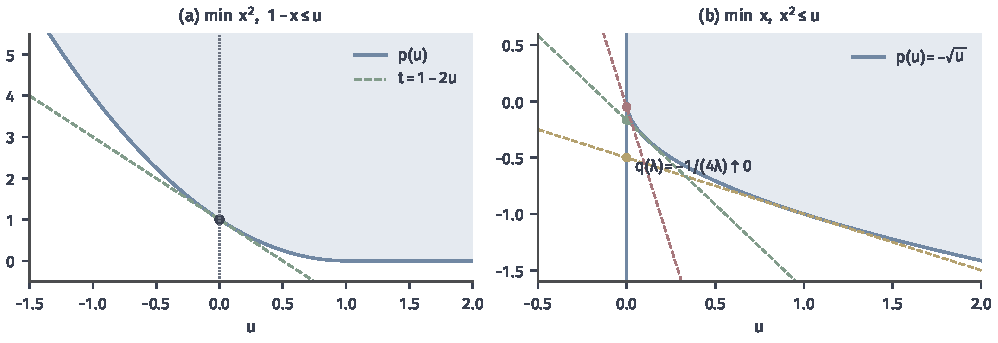
\includegraphics[width=169mm]{figures/03-optimization-evolution-and-signals/01-optimization/matplotlib/c5-slater/figure.pdf}
  \caption{扰动值函数$p(u)$与支撑直线。浅蓝区域为$p$的上图。(a) $\min x^2$、$1-x\leq u$：$p(u)=((1-u)_+)^2$，Slater点存在，绿色虚线$t=1-2u$在黑点$(0,1)$处支撑上图，斜率给出乘子$\lambda^\star=2$。(b) $\min x$、$x^2\leq u$：$u<0$不可行，$p(u)=-\sqrt u$在$u=0$处竖直；三条虚线是$\lambda=0.5,1.5,5$时的支撑直线，截距$q(\lambda)=-1/(4\lambda)$逐渐升向$0$，但没有有限斜率能达到。}
  \label{fig:opt-con-slater}
\end{figure*}

\paragraph{缺少条件时的反例}
线性规划的强对偶不能无条件推广。凸但不满足Slater条件的问题可以有正间隙：在定义域$x_2>0$上最小化$e^{-x_1}$，约束$x_1^2/x_2\leq0$。约束迫使$x_1=0$，故$f^\star=1$。而$\mathcal L=e^{-x_1}+\lambda x_1^2/x_2$，取$x_1=s$、$x_2=s^3$并令$s\to\infty$，得$\mathcal L\to0$，又$\mathcal L>0$，所以对每个$\lambda\geq0$都有$q(\lambda)=0$，$d^\star=0<1=f^\star$。约束函数$x_1^2/x_2$在$x_2>0$上凸，但它不可能严格小于零，Slater条件失败。非凸问题则可能有无穷大的间隙，如上一小节的$\min-x^2$，$x\in[-1,1]$。

\paragraph{KKT、零间隙与原始—对偶最优对}
下面的定理把第~\ref{sec:opt-con-optimality}节的候选检验与本节的界联系起来。

\begin{theorem}[零间隙与KKT条件]
\label{thm:opt-con-zero-gap-kkt}
(1) 若$\bm x^\star$可行、$\bm\lambda^\star\geq\bm0$且$f(\bm x^\star)=q(\bm\lambda^\star,\bm\nu^\star)$，则$\bm x^\star$是原问题的最优点，$(\bm\lambda^\star,\bm\nu^\star)$是对偶最优点，互补松弛成立，并且$\bm x^\star$是$\mathcal L(\cdot,\bm\lambda^\star,\bm\nu^\star)$的全局最小点；若各函数可微，则KKT条件成立。(2) 若原问题凸（$f,g_i$可微凸，$h_j$仿射）且$(\bm x^\star,\bm\lambda^\star,\bm\nu^\star)$满足KKT条件，则$f(\bm x^\star)=q(\bm\lambda^\star,\bm\nu^\star)$，两侧都最优。
\end{theorem}

\begin{proof}
(1) 由弱对偶，$f(\bm x^\star)=q(\bm\lambda^\star,\bm\nu^\star)\leq d^\star\leq f^\star\leq f(\bm x^\star)$，各处取等，两侧最优。又$q(\bm\lambda^\star,\bm\nu^\star)\leq\mathcal L(\bm x^\star,\bm\lambda^\star,\bm\nu^\star)=f(\bm x^\star)+\sum_i\lambda_i^\star g_i(\bm x^\star)\leq f(\bm x^\star)$，两端相等迫使$\sum_i\lambda_i^\star g_i(\bm x^\star)=0$；每一项非正，故逐项为零。同一串等式也说明$\mathcal L(\bm x^\star,\cdot)$达到下确界$q$，即$\bm x^\star$最小化$\mathcal L(\cdot,\bm\lambda^\star,\bm\nu^\star)$；可微时梯度为零，即驻点性。(2) 定理~\ref{thm:opt-con-kkt-sufficient}的证明已说明$\bm x^\star$最小化凸函数$\mathcal L(\cdot,\bm\lambda^\star,\bm\nu^\star)$，于是$q(\bm\lambda^\star,\bm\nu^\star)=\mathcal L(\bm x^\star,\bm\lambda^\star,\bm\nu^\star)=f(\bm x^\star)$。
\end{proof}

这条定理说明，在凸问题中“找到KKT点”与“找到零间隙的原始—对偶对”是同一件事。实际检验候选时仍要把几个问题分开：Slater条件或LICQ回答乘子是否存在；凸性回答KKT候选是否全局最优；原始最优点是否存在需要另外的紧性或强制性论证；而对于手中已有的有限精度候选，最可靠的是式~\eqref{eq:opt-con-gap-certificate}的上下界，它只依赖弱对偶。“强对偶成立”本身只是关于两个最优值的陈述，并不意味着已经找到了原始最优点。
